In the Laravel project, a straightforward REST API is implemented, offering a user-friendly interface for interacting with the Mosaico app store. The API endpoints are designed to be simple and intuitive:

\begin{center} \makebox[\textwidth]{ 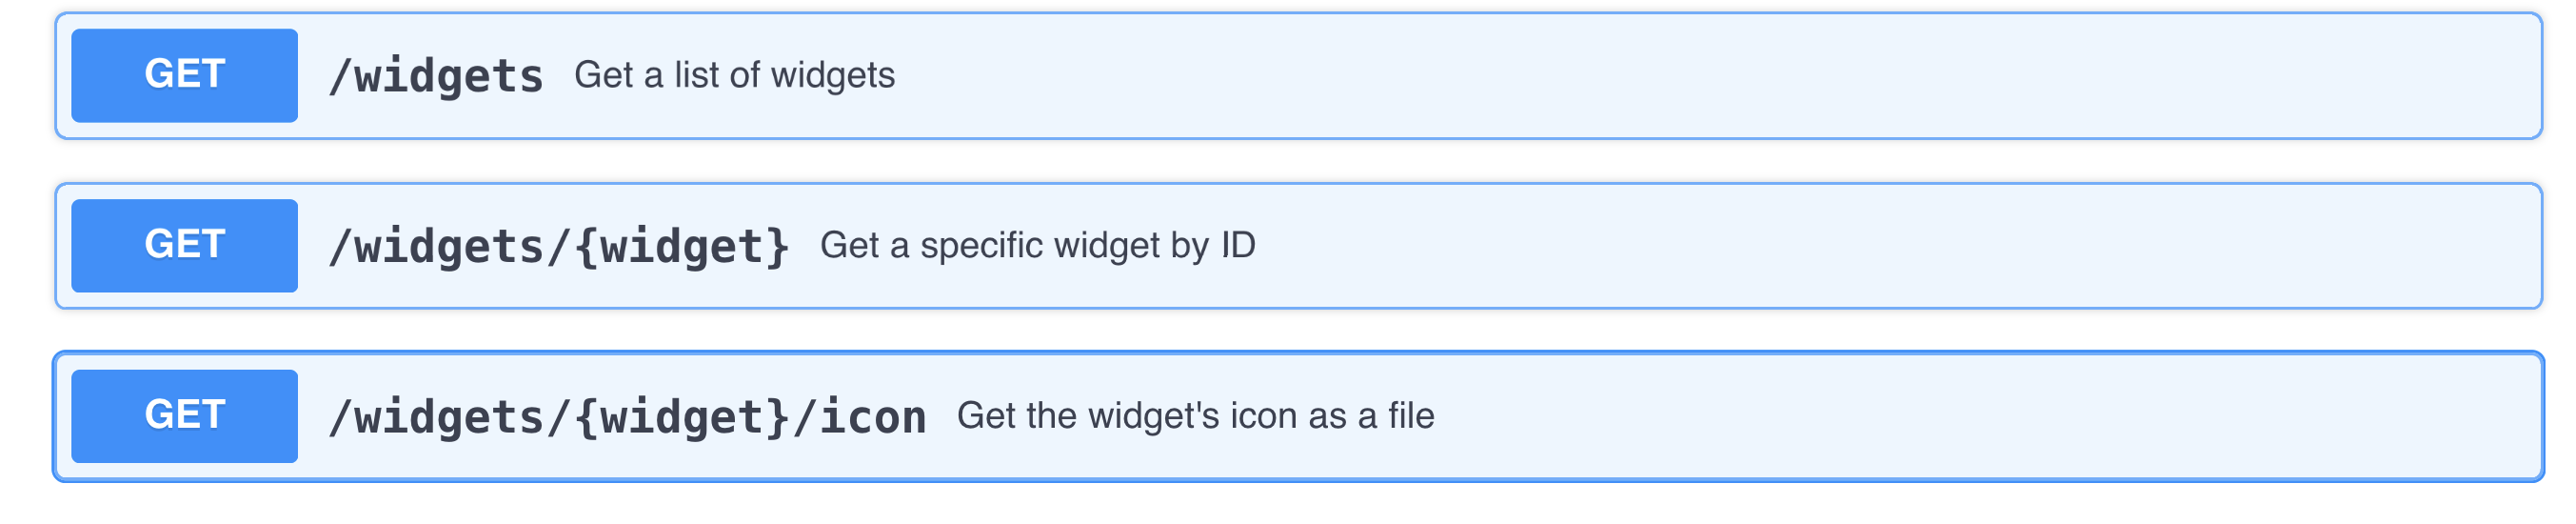
\includegraphics[width=0.8\paperwidth]{tesi/img/website_demo/api.png} } \end{center}

\subsection{Rate Limiter} Given that the only authenticated section of the application is the developer's dashboard, the API remains open for public access, allowing users to browse and utilize its features. However, this accessibility introduces potential vulnerabilities, such as Distributed Denial of Service (DDoS) attacks or spam requests. To mitigate these risks and protect the application’s logic as well as its database from excessive strain, a rate limiting mechanism has been implemented. This mechanism restricts the number of incoming requests from a specific IP address, effectively blocking those that exhibit suspicious behavior.